\section{\textit{K-Nearest Neighbors} (KNN)}
\label{sec:knn}

\todo{Satu paragraf pengantar: peran KNN dalam tugas ini dan ringkasan hasil terbaiknya.}

\subsection{Implementasi \textit{From Scratch}}
\label{subsec:knn-implementasi}

\subsubsection{Landasan Teori}
\todo{Jelaskan prinsip \textit{lazy learning}, metrik jarak (Euclidean, Manhattan, Minkowski), pemilihan $k$, \textit{voting} mayoritas atau berbobot jarak, dan penanganan \textit{tie}. Acu salindia KNN \cite{slide-knn} dan \cite{cunningham2020knn}. Sertakan rumus utama dalam lingkungan \texttt{equation}/\texttt{align}.}

\subsubsection{Struktur Kelas dan Fungsi}
\todo{Deskripsikan kelas pada \texttt{src/algoritma/knn/knn.py}: \texttt{\_\_init\_\_}, \texttt{fit}, perhitungan jarak, pencarian $k$ tetangga, \texttt{predict\_proba}, \texttt{predict}, \texttt{save}, \texttt{load}. Isi tabel di bawah, satu baris per fungsi/metode.}

\begin{table}[H]
	\centering
	\caption{Deskripsi kelas dan fungsi KNN}
	\label{tab:knn-fungsi}
	\begin{tabularx}{\textwidth}{l Y}
		\toprule
		\textbf{Fungsi/Metode} & \textbf{Deskripsi} \\
		\midrule
		\texttt{nama\_fungsi} & \todo{deskripsi} \\
		\bottomrule
	\end{tabularx}
\end{table}

\subsubsection{\textit{Source Code}}
\todo{Sisipkan potongan kode inti (perhitungan jarak (vektorisasi) dan \textit{voting}) dengan makro \texttt{\textbackslash kode}, lalu jelaskan alurnya. Cek ulang nomor baris jika kode berubah.}
% \kode{../../src/algoritma/knn/knn.py}{1}{30}{Judul potongan kode}{lst:knn-inti}

\subsubsection{\textit{Save} dan \textit{Load} Model}
\todo{Format penyimpanan (JSON/\texttt{.npz}/\textit{pickle}), isi yang disimpan, dan contoh pemakaian.}

\subsection{\textit{Data Cleaning} dan \textit{Preprocessing}}
\label{subsec:knn-preprocessing}

\todo{Jelaskan \textit{pipeline} khusus KNN beserta alasan tiap langkah, dikaitkan dengan temuan EDA (Subbab~\ref{sec:eda}) dan karakteristik algoritma. Semua transformasi di-\textit{fit} pada data latih saja lalu diterapkan ke data uji \cite{slide-dataprep}.}

\subsubsection{Penanganan \textit{Missing Values}}
\todo{KNN tidak bisa menghitung jarak dengan nilai hilang, sehingga imputasi wajib. Jelaskan strategi per kolom (median/modus/konstanta) dan alasannya.}

\subsubsection{Data Duplikat dan Data Tidak Valid}
\todo{Jumlah duplikat, nilai tidak wajar, atau \textit{outlier} yang ditangani untuk KNN dan caranya. Baris data uji tidak boleh dibuang.}

\subsubsection{Konstruksi Fitur dan \textit{Encoding}}
\todo{KNN butuh fitur numerik. Jelaskan \textit{encoding} kategorikal (\textit{one-hot} vs \textit{ordinal}/\textit{target}) dan dampaknya ke jarak (dimensi besar membuat jarak kurang bermakna).}

\subsubsection{Normalisasi dan Standarisasi}
\todo{Wajib karena KNN berbasis jarak. Fitur berskala besar akan mendominasi. Jelaskan \textit{scaler} yang dipilih (standar/\textit{min-max}/\textit{robust}).}

\subsubsection{Penanganan \textit{Imbalanced Data}}
\todo{Misalnya \textit{distance-weighted voting}, \textit{threshold} probabilitas, atau \textit{resampling}.}

\subsubsection{\textit{Feature Selection}}
\todo{Sangat berpengaruh karena fitur tak relevan ikut menambah jarak (\textit{curse of dimensionality}). Sebutkan fitur akhir yang dipakai.}

\subsubsection{\textit{Dimensionality Reduction}}
\todo{Relevan untuk KNN: mengurangi dimensi dan mempercepat perhitungan jarak. Laporkan dampaknya.}

\subsection{\textit{Modeling} dan Validasi}
\label{subsec:knn-validasi}

\subsubsection{Skema Validasi}
Setelah deduplikasi, sebanyak 27.309 baris dibagi secara \textit{stratified} dengan \textit{seed} 42 menjadi \textbf{21.847 data development} (80\%) dan \textbf{5.462 data holdout} (20\%). Seluruh pemilihan fitur dan hiperparameter dilakukan pada development. Data \textit{holdout} baru digunakan setelah konfigurasi ditentukan untuk memperoleh evaluasi yang terpisah dari proses pemilihan model.

Pada development, sepuluh kandidat fitur terlebih dahulu dibandingkan dengan \textit{stratified} 3-\textit{fold} CV. Dua representasi dengan Macro F1 tertinggi kemudian diuji dengan \textit{stratified} 5-\textit{fold} CV untuk mencari hiperparameter. Dalam setiap \textit{fold}, imputasi, normalisasi, dan kategori \textit{one-hot} di-\textit{fit} pada bagian latih saja. Nilai evaluasi yang dilaporkan adalah rata-rata Macro F1 tiap \textit{fold} beserta simpangan baku sampelnya. Skema ini menghindari kebocoran statistik \textit{preprocessing} dari \textit{fold} validasi, namun pemilihan dua kandidat awal dan pencarian parameter memakai development yang sama sehingga skor CV terbaik tetap merupakan hasil pemilihan model.

\subsubsection{\textit{Hyperparameter Tuning}}
Pencarian dilakukan atas dua representasi fitur, tujuh pilihan $k$, dan tiga metrik jarak. Total terdapat \textbf{42 konfigurasi}, semuanya menggunakan suara mayoritas tanpa pembobotan jarak. Ruang pencarian ditampilkan pada Tabel~\ref{tab:knn-grid}.

\begin{table}[H]
 \centering
 \caption{Ruang pencarian hiperparameter KNN}
 \label{tab:knn-grid}
 \begin{tabularx}{\textwidth}{l Y l}
  \toprule
  \textbf{Komponen} & \textbf{Kandidat} & \textbf{Terpilih} \\
  \midrule
  Representasi & 16 atau 15 fitur hasil seleksi & 16 fitur \\
  $k$ & 3, 5, 7, 9, 11, 15, 21 & 7 \\
  Metrik jarak & Manhattan, Euclidean, Minkowski ($p=3$) & Manhattan \\
  Pembobotan suara & \textit{Uniform} (tetap) & \textit{Uniform} \\
  \bottomrule
 \end{tabularx}
\end{table}

Hasil terbaik untuk setiap pasangan representasi dan metrik ditampilkan pada Tabel~\ref{tab:knn-tuning}. Nilai dalam tabel berasal dari berkas \nolinkurl{output/knn/tuning.csv}. Pada kombinasi yang diuji, konfigurasi 16 fitur dengan Manhattan $k=7$ memberikan rata-rata Macro F1 tertinggi, yaitu 0,82126.

\begin{table}[H]
 \centering
 \caption{Konfigurasi terbaik per representasi dan metrik pada 5-\textit{fold} CV}
 \label{tab:knn-tuning}
 \begin{tabular}{c l c c c}
  \toprule
  \textbf{Fitur} & \textbf{Jarak} & $\boldsymbol{k}$ & \textbf{Macro F1} & \textbf{SD} \\
  \midrule
  16 & Manhattan & 7 & \textbf{0,82126} & 0,00714 \\
  16 & Minkowski ($p=3$) & 7 & 0,82040 & 0,00721 \\
  16 & Euclidean & 7 & 0,82015 & 0,00724 \\
  15 & Minkowski ($p=3$) & 7 & 0,82013 & 0,00671 \\
  15 & Manhattan & 5 & 0,81955 & 0,00663 \\
  15 & Euclidean & 7 & 0,81869 & 0,00669 \\
  \bottomrule
 \end{tabular}
\end{table}

\begin{figure}[H]
 \centering
 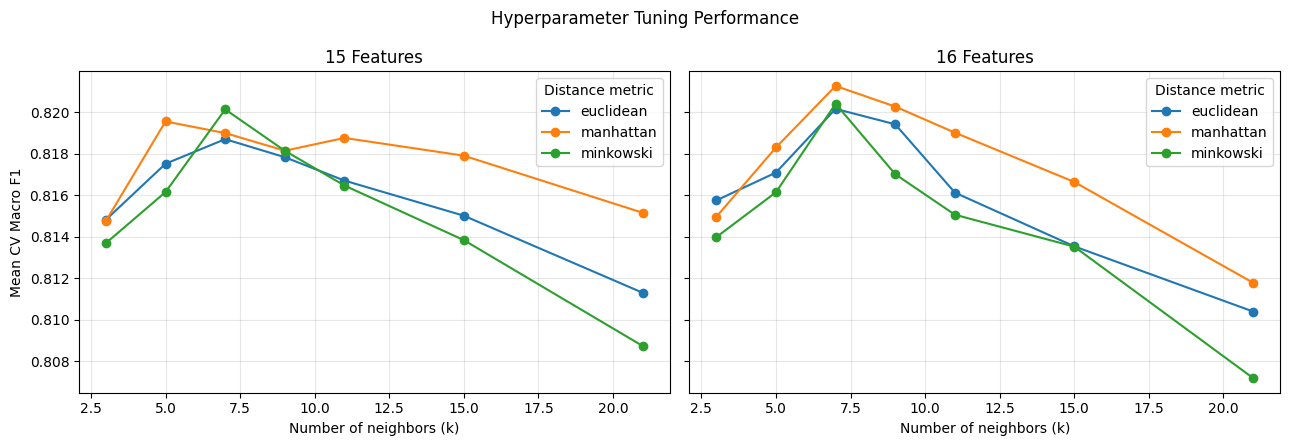
\includegraphics[width=0.94\textwidth]{knn/knn_tuning.png}
 \caption{Rata-rata Macro F1 validasi silang menurut $k$ dan metrik jarak pada dua representasi fitur}
 \label{fig:knn-tuning}
\end{figure}

Gambar~\ref{fig:knn-tuning} menunjukkan bahwa kinerja berubah ketika jumlah tetangga atau metrik jarak diganti. Perbedaan antar konfigurasi terbaik relatif kecil, yaitu 0,00086 antara Manhattan dan Minkowski pada 16 fitur. Nilai ini juga lebih kecil daripada simpangan baku antar-\textit{fold} sekitar 0,007. Oleh sebab itu, konfigurasi terbaik dipahami sebagai pilihan berdasarkan rata-rata pada ruang pencarian yang diuji, bukan bukti keunggulan yang pasti untuk semua pembagian data.

\subsubsection{Model Final}
KNN final menggunakan \textbf{16 fitur, Manhattan, $k=7$, dan suara mayoritas uniform}. Skor development CV adalah $\text{Macro F1}=0{,}82126\pm0{,}00714$, dengan \textit{accuracy} rata-rata 0,84552. Kelima skor Macro F1 per \textit{fold} adalah 0,82781, 0,81894, 0,81019, 0,82685, dan 0,82251. Model kemudian di-\textit{fit} pada seluruh development dan dievaluasi sekali pada \textit{holdout}, sebagaimana dibahas pada Subbab~\ref{subsec:knn-hasil}.

Untuk membuat prediksi data uji, konfigurasi yang sama di-\textit{fit} ulang pada \textbf{27.309 data latih bersih}. Pipeline menyimpan model dan statistik \textit{preprocessing} di \nolinkurl{output/knn/model.pkl}, hasil pencarian di \nolinkurl{output/knn/tuning.csv}, dan prediksi \textbf{6.844 baris} di \nolinkurl{output/knn/submission.csv}. Artefak tersebut dapat direproduksi melalui \nolinkurl{src/kaggle/knn_notebook.ipynb} atau \nolinkurl{src/kaggle/knn_submission.py}.
\subsection{Hasil dan Perbandingan dengan \textit{Scikit-learn}}
\label{subsec:knn-hasil}

Model terpilih dibandingkan dengan \texttt{sklearn.neighbors.KNeighborsClassifier} \cite{pedregosa2011sklearn} pada \textbf{data holdout yang sama}. Kedua implementasi menerima matriks 26 kolom yang sama dari \textit{preprocessor} yang hanya di-\textit{fit} pada development. Parameter pembanding disamakan, yaitu $k=7$, Manhattan, bobot \textit{uniform}, dan pencarian \textit{brute force}. Dengan demikian, pengujian memeriksa konsistensi hasil prediksi implementasi \textit{from scratch}, bukan perbedaan akibat pemrosesan data.

\begin{table}[H]
 \centering
 \caption{Perbandingan performa KNN pada 5.462 reservasi \textit{holdout}}
 \label{tab:knn-hasil}
 \begin{tabular}{l c c c c}
  \toprule
  \textbf{Implementasi} & \textbf{Macro F1} & \textbf{Accuracy} & \textbf{Macro Precision} & \textbf{Macro Recall} \\
  \midrule
  \textit{From scratch} & 0,82830 & 0,85244 & 0,83803 & 0,82075 \\
  \textit{Scikit-learn} & 0,82830 & 0,85244 & 0,83803 & 0,82075 \\
  \bottomrule
 \end{tabular}
\end{table}

\textbf{Seluruh 5.462 prediksi identik} antara kedua implementasi, sehingga kesesuaian label mencapai 100\%. Confusion matrix keduanya sama, sebagaimana ditampilkan pada Gambar~\ref{fig:knn-cm}. Hasil ini mendukung ketepatan implementasi jarak dan suara mayoritas pada konfigurasi serta data yang diuji. Kesamaan prediksi tersebut tidak berarti seluruh kemungkinan \textit{tie} jarak akan selalu ditangani identik oleh kedua implementasi.

\begin{figure}[H]
 \centering
 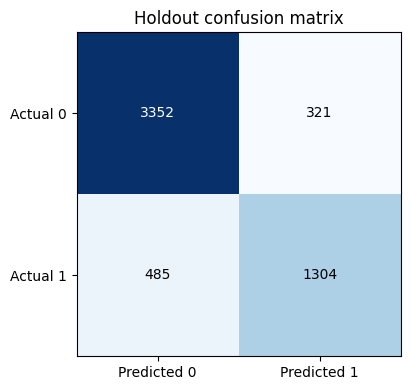
\includegraphics[width=0.66\textwidth]{knn/knn_confusion_matrix.png}
 \caption{\textit{Confusion matrix} KNN \textit{from scratch} pada \textit{holdout}, identik dengan \textit{scikit-learn}}
 \label{fig:knn-cm}
\end{figure}

\subsubsection{Analisis}
Dari 3.673 reservasi yang sebenarnya tidak dibatalkan, model mengklasifikasikan 3.352 dengan benar dan menghasilkan 321 \textit{false positive}. Dari 1.789 reservasi yang dibatalkan, model mengenali 1.304 dengan benar dan melewatkan 485 sebagai \textit{false negative}. \textit{Recall} kelas batal sebesar 0,72890 lebih rendah daripada kelas tidak batal sebesar 0,91261. Dengan demikian, kelemahan utama KNN pada \textit{holdout} adalah pembatalan yang tidak terdeteksi, bukan ketidakcocokan implementasi dengan pustaka.

Skor Macro F1 \textit{holdout} sebesar 0,82830 sedikit di atas rata-rata CV development 0,82126. Keduanya berada pada kisaran yang sebanding, meskipun berasal dari skema evaluasi berbeda. Peningkatan kemampuan mengenali kelas batal berpotensi dilakukan melalui kalibrasi ambang keputusan atau pembobotan fitur, tetapi perubahan tersebut tidak diterapkan pada model utama. Dalam konteks bonus biaya kesalahan, FP justru memiliki konsekuensi lebih mahal sehingga arah penyesuaian keputusan juga berbeda, seperti dibahas pada Subbab~\ref{subsec:knn-bonus}.

Pengukuran waktu prediksi tidak dilakukan sebagai eksperimen pembanding, sehingga tidak ditarik kesimpulan mengenai kecepatan kedua implementasi. Versi \textit{from scratch} memakai \texttt{cdist} dan \texttt{argpartition} dengan \textit{batch} untuk membatasi memori sementara. Pembanding \textit{scikit-learn} secara eksplisit memakai \textit{brute force} agar metode pencarian tetangganya sebanding.
\subsection{Analisis \textit{Cost-Sensitive Classification} pada KNN}
\label{subsec:knn-bonus}

Bonus \textit{cost-sensitive classification} pada spesifikasi menetapkan bahwa \textit{false positive} (FP) dua kali lebih mahal dibandingkan \textit{false negative} (FN). Dalam kasus reservasi, FP berarti model memprediksi pembatalan padahal tamu tetap datang, sehingga keputusan menjual ulang kamar dapat menimbulkan \textit{overbooking}. Konsekuensinya, penanganan klasifikasi perlu lebih berhati-hati dalam memberikan label batal. Asumsi biaya yang sama juga dibahas pada tingkat kelompok di Subbab~\ref{sec:cost-sensitive}.

\subsubsection{Perubahan Aturan Keputusan}
Dengan biaya prediksi benar nol, $C_{FP}=2$, dan $C_{FN}=1$, total biaya kesalahan didefinisikan sebagai
\begin{equation}
 C_{\mathrm{total}} = 2FP + FN.
 \label{eq:knn-cost}
\end{equation}
Jika $p$ merupakan estimasi peluang kelas batal, biaya harapan ketika memilih kelas batal adalah $2(1-p)$, sedangkan ketika memilih kelas tidak batal adalah $p$. Aturan yang meminimalkan biaya harapan memilih batal jika
\begin{equation}
 2(1-p)\le p \quad\Longleftrightarrow\quad p\ge\frac{2}{3}.
 \label{eq:knn-threshold}
\end{equation}
Pada KNN, nilai $p$ diestimasi dari proporsi suara tetangga melalui \texttt{predict\_proba}. Untuk $k=7$, aturan mayoritas biasa memerlukan sedikitnya empat tetangga berlabel batal. Ambang $2/3$ mengubah syarat tersebut menjadi \textbf{minimal lima tetangga}. Proporsi suara KNN belum dikalibrasi sebagai probabilitas, sehingga rumus ini dipakai sebagai kebijakan berbasis asumsi biaya yang kemudian diperiksa secara empiris, bukan sebagai jaminan optimum global \cite{elkan2001cost}.

\subsubsection{Hasil dan Analisis}
Simulasi dilakukan pada \textit{holdout} berukuran 5.462 menggunakan konfigurasi 16 fitur, Manhattan, dan $k=7$ yang sama dengan model utama. KNN di-\textit{fit} hanya pada development. Aturan baru diterapkan pada proporsi suara kelas batal tanpa mengubah data latih, hasil \textit{feature selection}, maupun berkas submisi.

\begin{table}[H]
 \centering
 \caption{Perbandingan keputusan KNN standar dan \textit{cost-sensitive} pada \textit{holdout}}
 \label{tab:knn-cost}
 \begin{tabular}{l r r r c}
  \toprule
  \textbf{Aturan keputusan} & \textbf{FP} & \textbf{FN} & \textbf{Total biaya} & \textbf{Macro F1} \\
  \midrule
  Mayoritas standar, minimal 4/7 & 321 & 485 & 1.127 & 0,82830 \\
  \textit{Cost-sensitive}, minimal 5/7 & 177 & 673 & \textbf{1.027} & 0,80791 \\
  \bottomrule
 \end{tabular}
\end{table}

\begin{figure}[H]
 \centering
 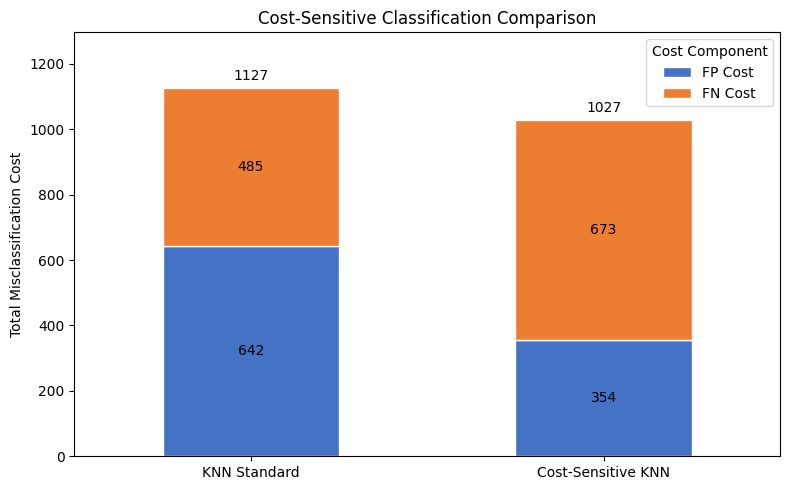
\includegraphics[width=0.72\textwidth]{knn/knn_cost_sensitive.png}
 \caption{Komponen biaya FP dan FN pada aturan mayoritas standar dan \textit{cost-sensitive}}
 \label{fig:knn-cost}
\end{figure}

Perubahan ambang mengurangi FP sebanyak 144 tetapi menambah FN sebanyak 188. Karena satu FP bernilai dua unit biaya, pengurangan FP menghemat 288 unit, sedangkan tambahan FN menambah 188 unit. Biaya bersih turun \textbf{100 unit}, dari 1.127 menjadi 1.027 atau \textbf{8,87\%}. Pada saat yang sama, Macro F1 turun dari 0,82830 menjadi 0,80791. Hasil tersebut menunjukkan bahwa aturan yang lebih sesuai dengan biaya bisnis tidak harus memaksimalkan Macro F1.

Analisis ini merupakan evaluasi tambahan, bukan pelatihan model baru dan bukan submisi Kaggle baru. \texttt{output/knn/submission.csv} tetap memakai keputusan mayoritas standar karena metrik kompetisi adalah Macro F1. Evaluasi dilakukan pada \textit{holdout} yang tidak dipakai memilih ambang $2/3$, sehingga perbandingan memberikan bukti langsung tentang dampak aturan biaya pada konfigurasi KNN yang sudah dipilih.
